% Adapted from: https://texample.net//tikz/examples/events/
\documentclass[border=5pt]{standalone}

\usepackage[utf8]{inputenc}
\usepackage{garamondx}

\usepackage[x11names]{xcolor}
\usepackage{xfp}
\usepackage{tikz}
\usetikzlibrary{arrows, positioning}

\tikzstyle{basefont}=[font=\Large] %\sffamily
\tikzstyle{timing}=[basefont, sloped, above]
\tikzstyle{label}=[basefont, align=left]
\tikzstyle{screen}=[basefont, white, align=center, minimum size=6cm, fill=black!60, draw=white]
\tikzstyle{arrow}=[ultra thick, ->, >=latex]

\newcommand*{\screen}[4]{%
	\def\yslant{0.33}
	\begin{scope}[xshift=#3, yshift=#4,
                  every node/.append style={yslant=\yslant},
                  yslant=\yslant, local bounding box=#1]
   		\node[screen] at (3cm, 3cm) {#2};
    \end{scope}
}

\begin{document}
	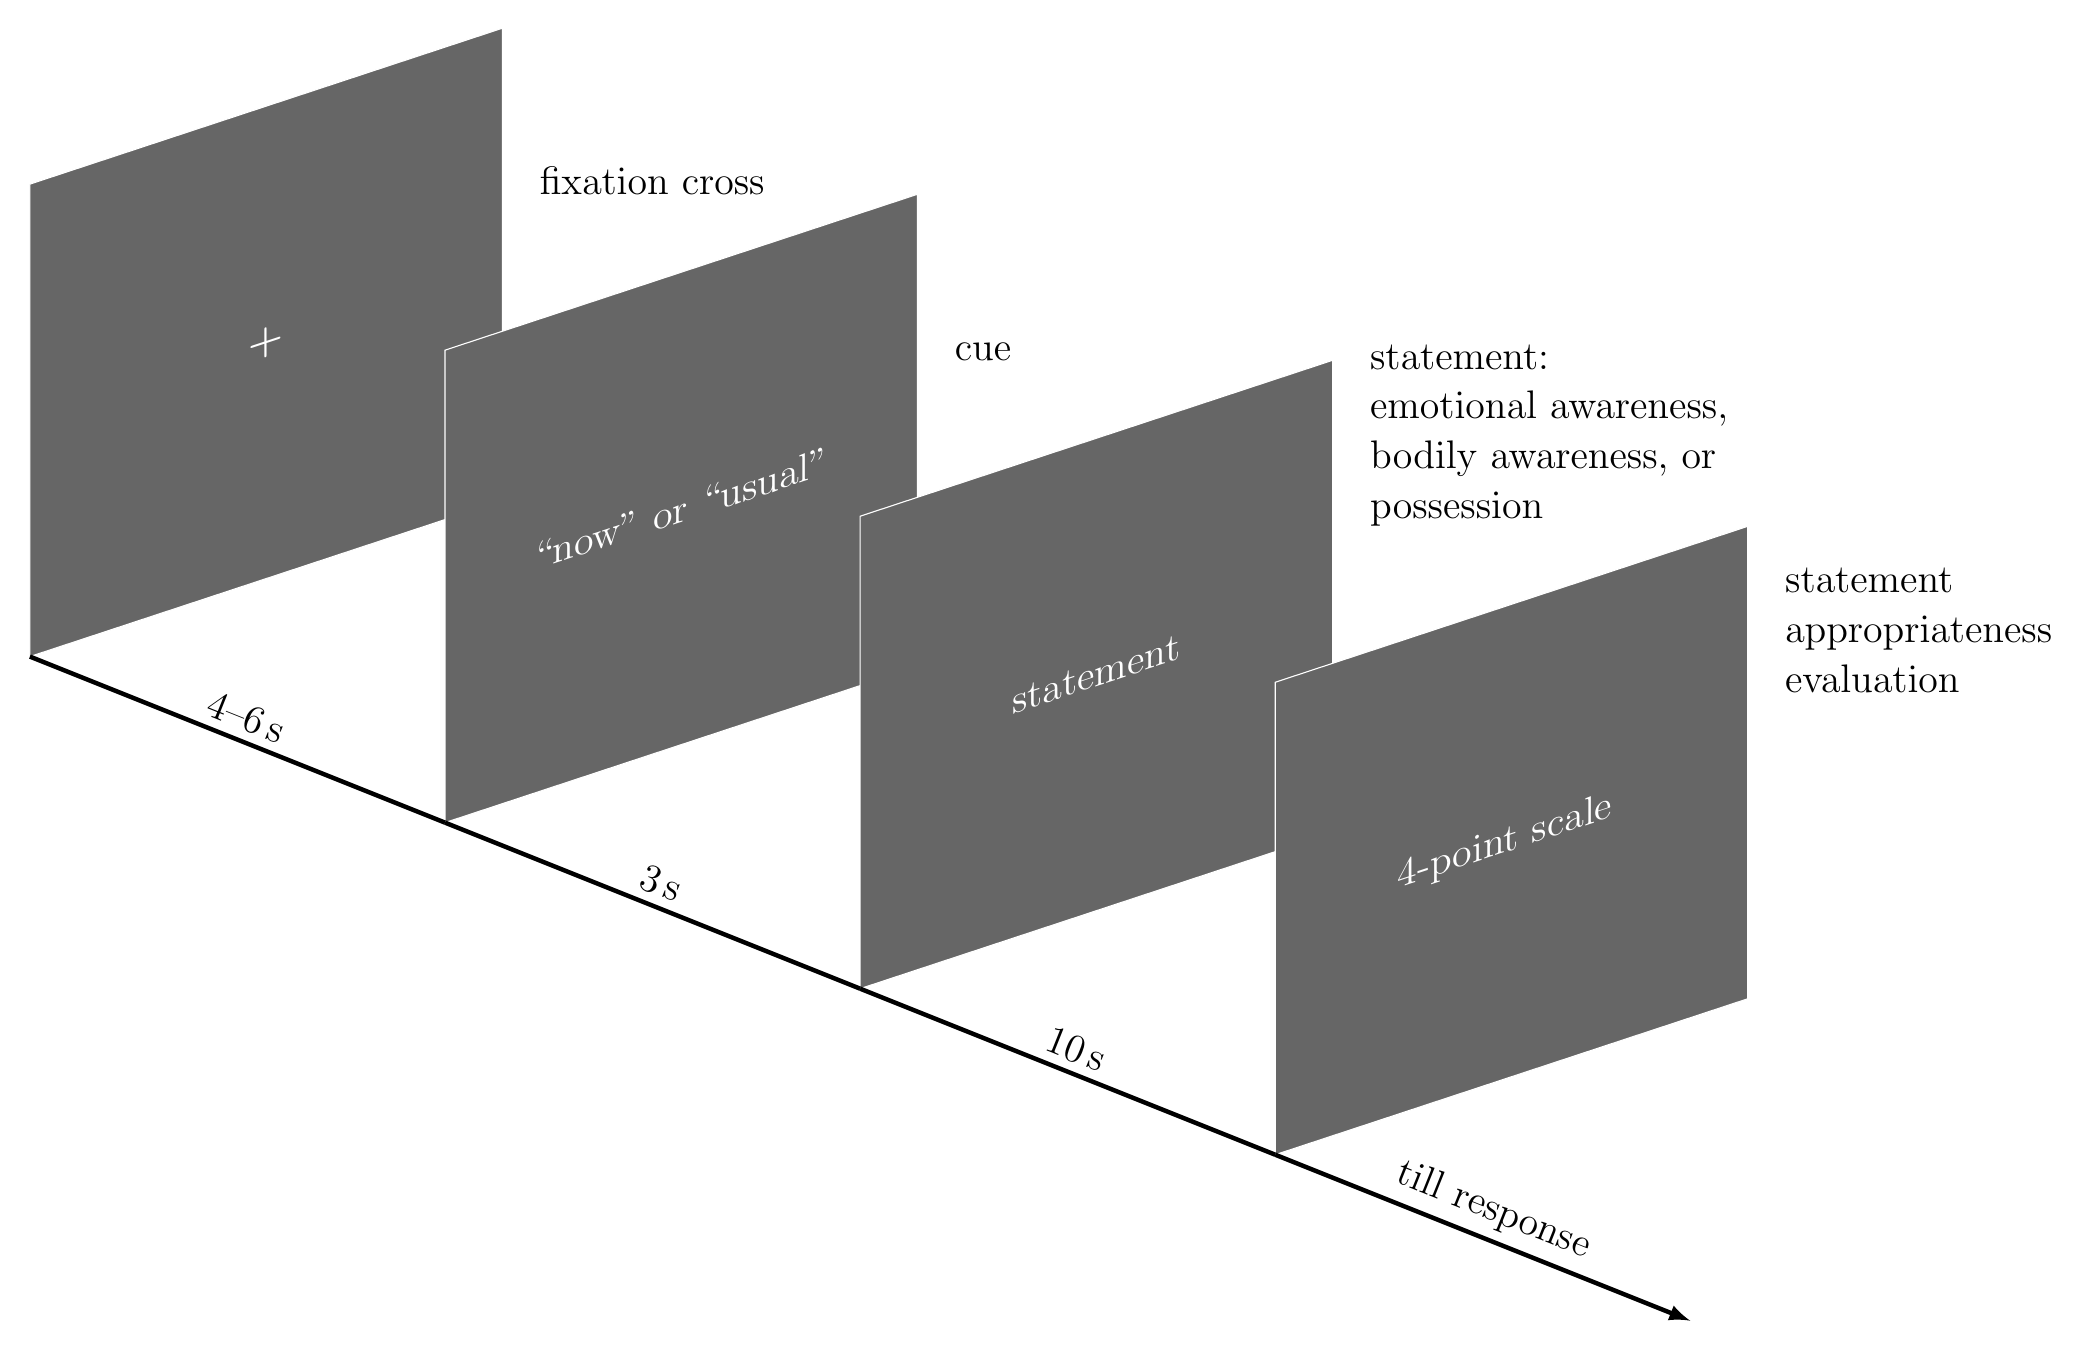
\begin{tikzpicture}[node distance=3em]
        % Define several screens
        \def\xstep{150}
        \def\ystep{-60}
        \def\nscreens{0}
        \foreach \content [count=\i] in {
        	\textbf{+},
			``now'' or ``usual'',
			statement,
			4-point scale
        }{
        	% https://tex.stackexchange.com/a/520694/181375
			\pgfmathtruncatemacro\j{\i-1}
			\pgfmathtruncatemacro\x{\j*\xstep}
			\pgfmathtruncatemacro\y{\j*\ystep}
			
			% Create screen
        	\screen{frame\i}{\content}{\x}{\y}
			
			% Update screen counter
			% https://tex.stackexchange.com/a/115428/181375
			\xdef\nscreens{\i}
        }
        
        % Add phantom coordinate after last screen
        % https://tex.stackexchange.com/a/66849/181375
        % https://tex.stackexchange.com/a/437021/181375
		\pgfmathtruncatemacro\x{\nscreens*\xstep}
		\pgfmathtruncatemacro\y{\nscreens*\ystep}
        \coordinate [xshift=\x, yshift=\y] (frame\the\numexpr\nscreens+1);

        % Add annotations to screens
        \foreach \content [count=\i] in {
            fixation cross,
            cue,
            statement:\\{emotional awareness,}\\{bodily awareness,} or\\possession,
            statement\\appropriateness\\evaluation
        }{
            \node[label, above right=5em and 1em of frame\i.east]
            (f\i-label) {\content};
        }

        % Add time course line and labels
        \foreach \content [count=\i] in {
            $4$--$6$\,s,
            $3$\,s,
            $10$\,s,
            till response
        }{
            \tikzset{
            	timepath/.style={ultra thick},
				last/.code={
    				% Need to draw an arrow if at end of loop
					% https://tex.stackexchange.com/a/214996/181375
    				\ifnum##1=\the\numexpr\nscreens+1\tikzset{timepath, arrow}\fi
				}
			}
			
			\pgfmathtruncatemacro\j{\i+1}
            \path[timepath, last=\j] (frame\i.south west) edge
            node[timing] {\content} (frame\j.south west);
        }
	\end{tikzpicture}
\end{document}
